%%%%%%%%%%%%%%%%%%%%%%%%%%%%%%%%%%%%%%%%%%%%%%%%%%%%%%%%%%%%%%%%%%%%%%%%%%%%%%%%
% DOCUMENT SPECIFICATION
%%%%%%%%%%%%%%%%%%%%%%%%%%%%%%%%%%%%%%%%%%%%%%%%%%%%%%%%%%%%%%%%%%%%%%%%%%%%%%%%
% \documentclass[twoside,a4paper]{scrartcl}        % Koma-script class
\documentclass[a4paper]{scrartcl}               % Koma-script class

%----------------------------------------------------------------------------------------
% PREAMBLE: PACKAGES AND CONFIGURATIONS
%----------------------------------------------------------------------------------------
% !TEX root = main.tex
%
% TODO: Have a clearer separation between ZHAW Thesis class and this preamble.

%%%%%%%%%%%%%%%%%%%%%%%%%%%%%%%%%%%%%%%%%%%%%%%%%%%%%%%%%%%%%%%%%%%%%%%%%%%%%%%%
% Fonts and characters
%%%%%%%%%%%%%%%%%%%%%%%%%%%%%%%%%%%%%%%%%%%%%%%%%%%%%%%%%%%%%%%%%%%%%%%%%%%%%%%%

% Support for special characters
\usepackage[utf8]{inputenc}    % Input encoding: Support non-ascii characters
\usepackage[T1]{fontenc}       % Font encoding: T1 is good choice for Europe

% Set main fonts
% Fonts catalogue: https://tug.org/FontCatalogue/
\usepackage{mathpazo}          % Use the Palatino font by default
\usepackage{beramono}          % Override the monospace/typewriter font

\usepackage{amssymb}           % Maths
\usepackage{amsmath}           % Maths 
\usepackage{numprint}          % For nicely printing large numbers
\usepackage{lmodern}           % Use LaTeX math fonts, requires T1
\usepackage[normalem]{ulem}    % Strikethrough text.

\usepackage{pdfpages}

% ZHAW title font
% Try to load Helvetica Rounded Bold, and OpenType font.
% Loading OTF or system fonts is possible with XeLaTeX.
% If the document is compiled using pdfLaTeX, resort 
\usepackage{ifxetex}
\ifxetex
    \usepackage{fontspec}
    \newfontfamily\zhawtitlefont{Helvetica Rounded Bold}
\else
    \newcommand{\zhawtitlefont}{\scshape}
\fi

\newcommand{\boldit}[1]{\textit{\textbf{#1}}}

% Set Helvetica as the default font
\usepackage[scaled]{helvet}
\renewcommand{\familydefault}{\sfdefault}

%%%%%%%%%%%%%%%%%%%%%%%%%%%%%%%%%%%%%%%%%%%%%%%%%%%%%%%%%%%%%%%%%%%%%%%%%%%%%%%%
% Comments
%%%%%%%%%%%%%%%%%%%%%%%%%%%%%%%%%%%%%%%%%%%%%%%%%%%%%%%%%%%%%%%%%%%%%%%%%%%%%%%%

\usepackage[color=cyan,colorinlistoftodos]{todonotes}
\newcommand{\replace}[2]{{\sout{#1}} \textcolor{cyan}{#2}}
\newcommand{\note}[1]{\textcolor{cyan}{#1}}

%%%%%%%%%%%%%%%%%%%%%%%%%%%%%%%%%%%%%%%%%%%%%%%%%%%%%%%%%%%%%%%%%%%%%%%%%%%%%%%%
% Colors
%%%%%%%%%%%%%%%%%%%%%%%%%%%%%%%%%%%%%%%%%%%%%%%%%%%%%%%%%%%%%%%%%%%%%%%%%%%%%%%%

% Set up colors
\usepackage[dvipsnames]{xcolor} % Color management
% \PassOptionsToPackage{dvipsnames}{xcolor}  % Had to change this.

% ZHAW Blue: Pantone 2945 U / R0 G100 B166
\definecolor{zhawblue}{rgb}{0.00, 0.39, 0.65}
\definecolor{zhawlightblue}{rgb}{0.82, 0.88, 0.93}
% Colors related to code listings
\definecolor{codegreen}{rgb}{0,0.6,0}
\definecolor{codegray}{rgb}{0.5,0.5,0.5}
\definecolor{codepurple}{rgb}{0.58,0,0.82}
\definecolor{codebackground}{rgb}{0.93,0.94,0.95}
% Colors related to tables
\definecolor{tablegray}{rgb}{0.9,0.9,0.9}
\colorlet{tableheader}{tablegray}
% Colors related to hyperref
\definecolor{linkcolor}{rgb}{0.00, 0.39, 0.65}
\definecolor{urlcolor}{rgb}{0.00, 0.39, 0.65}

%%%%%%%%%%%%%%%%%%%%%%%%%%%%%%%%%%%%%%%%%%%%%%%%%%%%%%%%%%%%%%%%%%%%%%%%%%%%%%%%
% Environments
%%%%%%%%%%%%%%%%%%%%%%%%%%%%%%%%%%%%%%%%%%%%%%%%%%%%%%%%%%%%%%%%%%%%%%%%%%%%%%%%

% \usepackage[ngerman]{babel}   % Language support
\usepackage[english]{babel}     % Language support
\usepackage[                    % Create hypertext links
    colorlinks=true, 
    allbordercolors={white}, 
    linkcolor=linkcolor,
    citecolor=linkcolor, 
    filecolor=linkcolor,
    linktoc=all, 
    urlcolor=urlcolor
    ]{hyperref}

\usepackage{xurl}              % Superior to url or breakurl for breaking long URLs
\usepackage{graphicx}          % Include graphics
\usepackage{float}             % Improved interface for floating objects
\usepackage{tabularx}          % Create nicer tables
\usepackage{multirow}          % Merge rows in tables
\usepackage{booktabs}          % To further beautify tables
\usepackage{longtable}         % For tables that span multiple pages
\usepackage{caption}           % Customized caption
\usepackage{subcaption}        % Subfigure captions
\usepackage{makecell}          % Per-cell formatting in tables (\makecell)
\usepackage{pdfpages}          % Required to include PDF files/graphics (\includepdf)
\usepackage{colortbl}          % Tables with colors
\usepackage[tooltip]{acro}     % For acronyms and abbreviations
\usepackage[autostyle=true]{csquotes} 
                               % Required to generate language-dependent quotes 
                               % in the bibliography
  
\usepackage{todonotes}         % Introduces the command \todo
\setlength{\marginparwidth}{2.5cm} % Adjust this if the todo notes are out of margins
\usepackage{array,ragged2e}    % For ragged alignment of multi-line table cells

% Adjust tables
\colorlet{tableheadcolor}{gray!25}                % Table header colour
\newcommand{\headcol}{\rowcolor{tableheadcolor}}% % The color of the head
\newcommand{\topline}{\arrayrulecolor{black}      %
                      \specialrule{0.1em}{\abovetopsep}{0.5pt}%
                      \arrayrulecolor{tableheadcolor}%
                      \specialrule{\belowrulesep}{0pt}{-3pt}%
            \arrayrulecolor{black}
            }
\newcommand{\midline}{\arrayrulecolor{tableheadcolor}
            \specialrule{\aboverulesep}{-1pt}{0pt}%
            \arrayrulecolor{black}\specialrule{\lightrulewidth}{0pt}{0pt}%
            \arrayrulecolor{white}\specialrule{\belowrulesep}{0pt}{-3pt}%
            \arrayrulecolor{black}
            }
\newcommand{\bottomline}{\arrayrulecolor{white}\specialrule{\aboverulesep}{0pt}{-2pt}%
            \arrayrulecolor{black}\specialrule{\heavyrulewidth}{0pt}{\belowbottomsep}}%

% Create boxes as follows:
% \begin{colorbox}{red}{2}
\usepackage{tcolorbox}
\newtcolorbox{textbox}[2]{
    arc=3pt,
    boxrule=#2pt,
    colback=#1!25!white,
    width=\textwidth,
    halign=left,
    valign=center,
    colframe=#1!75!black
}

%%%%%%%%%%%%%%%%%%%%%%%%%%%%%%%%%%%%%%%%%%%%%%%%%%%%%%%%%%%%%%%%%%%%%%%%%%%%%%%%
% Code listings
%%%%%%%%%%%%%%%%%%%%%%%%%%%%%%%%%%%%%%%%%%%%%%%%%%%%%%%%%%%%%%%%%%%%%%%%%%%%%%%%
\captionsetup{format=plain,             % plain or hang
              justification=justified,  % justified, centering, raggedright, ...
              labelfont=bf,
              font=small,
              margin=20pt}
              

%%%%%%%%%%%%%%%%%%%%%%%%%%%%%%%%%%%%%%%%%%%%%%%%%%%%%%%%%%%%%%%%%%%%%%%%%%%%%%%%
% Code listings
%%%%%%%%%%%%%%%%%%%%%%%%%%%%%%%%%%%%%%%%%%%%%%%%%%%%%%%%%%%%%%%%%%%%%%%%%%%%%%%%

\newcommand{\code}[1]{\texttt{#1}}



% Setup code listings
\usepackage{listings}
\lstdefinestyle{mystyle}{
    backgroundcolor=\color{codebackground},   
    commentstyle=\color{codegreen},
    keywordstyle=\color{magenta},
    numberstyle=\tiny\color{codegray},
    stringstyle=\color{codepurple},
    basicstyle=\ttfamily\scriptsize,
    breakatwhitespace=false,
    breaklines=true,
%    captionpos=b,
    keepspaces=true,
    numbers=left,
    numbersep=5pt,
    showspaces=false,
    showstringspaces=false,
    showtabs=false,
    tabsize=4
}
\lstset{style=mystyle}

% minted is an alternative code listing package. (See appendix A)
% For it to run successfully, ensure the following:
% - the Python package Pygments. Install with the following command:
%       python -m pip install Pygments
% - pdflatex (or xelatex) is executed with the flag --shell-escape
%   If you are using a TEX editor, you can modify the typesetting 
%   command somewhere in the settings.
%\usepackage[outputdir=build]{minted}
%\usemintedstyle{xcode}
% For fancier coloring schemes, see here:
% https://tex.stackexchange.com/questions/585582
% One could also create an own style in Pygments
% https://pygments.org/docs/styles/#creating-own-styles

%%%%%%%%%%%%%%%%%%%%%%%%%%%%%%%%%%%%%%%%%%%%%%%%%%%%%%%%%%%%%%%%%%%%%%%%%%%%%%%%
% MARGIN SETTINGS
%%%%%%%%%%%%%%%%%%%%%%%%%%%%%%%%%%%%%%%%%%%%%%%%%%%%%%%%%%%%%%%%%%%%%%%%%%%%%%%%
\usepackage{geometry}
\geometry{
    paper=a4paper,       % Change to letterpaper for US letter
    %inner=2.5cm,        % Inner margin
    %outer=3.8cm,        % Outer margin
    %top=1.5cm,          % Top margin
    bottom=4.cm,         % Bottom margin
    bindingoffset=.5cm,  % Binding offset
    %showframe,          % Show the type block of the page
}

% Other layout settings
\setlength\parindent{0em} % No indent
\setlength{\parskip}{1em}
%\usepackage{parskip}


\setlength{\intextsep}{30pt}   % Distance between image and text 
\usepackage{enumitem}          % Layout control for list environments (e.g, itemize)
\setlist{noitemsep}            % Suppress extra spaces between items
%\setlist{nosep}               % Suppress spaces before/after list environments


%----------------------------------------------------------------------------------------
%   PENALTIES
%----------------------------------------------------------------------------------------

\doublehyphendemerits=10000 % No consecutive line hyphens
\brokenpenalty=10000 % No broken words across columns/pages
\widowpenalty=9999 % Almost no widows at bottom of page
\clubpenalty=9999 % Almost no orphans at top of page
\interfootnotelinepenalty=9999 % Almost never break footnotes


%%%%%%%%%%%%%%%%%%%%%%%%%%%%%%%%%%%%%%%%%%%%%%%%%%%%%%%%%%%%%%%%%%%%%%%%%%%%%%%%
% MANAGE AUTHOR LISTS
%%%%%%%%%%%%%%%%%%%%%%%%%%%%%%%%%%%%%%%%%%%%%%%%%%%%%%%%%%%%%%%%%%%%%%%%%%%%%%%%

\usepackage[affilmode=count]{authors}


% Trick: Convert the setter into a getter.
\NewDocumentCommand{\pdfautorstring}{m}{\renewcommand{\pdfautorstring}{#1}}
\NewDocumentCommand{\projecttitle}{m}{\renewcommand{\projecttitle}{#1}}
\NewDocumentCommand{\projecttype}{m}{\renewcommand{\projecttype}{#1}}
\NewDocumentCommand{\projectcode}{m}{\renewcommand{\projectcode}{#1}}
\NewDocumentCommand{\projectdate}{m}{\renewcommand{\projectdate}{#1}}
\NewDocumentCommand{\keywords}{m}{\renewcommand{\keywords}{#1}}

\NewDocumentCommand{\university}{m}{\renewcommand{\university}{#1}}
\NewDocumentCommand{\department}{m}{\renewcommand{\department}{#1}}
\NewDocumentCommand{\institute}{m}{\renewcommand{\institute}{#1}}
\NewDocumentCommand{\group}{m}{\renewcommand{\group}{#1}}


%----------------------------------------------------------------------------------------
%   HEADERS AND FOOTERS
%----------------------------------------------------------------------------------------

% Notes:
% - In twoside mode, left and right side pages may differ
% - Pages: left = even, right = odd
%   Chapters usually are forced to start at odd pages.
% - \markboth{left}{right} how left and right pages are marked
% - \automark is a convenience command from the scrlayer-scrpage package. It issues 
%   that \markboth is called for every \chapter and \section command.
% - Historical note: scrlayer-scrpage is the successor of scrpage2
% - Refs:
%    \markboth:  https://tex.stackexchange.com/questions/198676
%    \automark:  https://tex.stackexchange.com/questions/34269/
%    \automark*: https://tex.stackexchange.com/questions/348550/
%
\usepackage[markcase=used]{scrlayer-scrpage}
\ifoot{}% Empty inner footer by default
\ofoot{}% Empty outer footer by default
\providepairofpagestyles{basicStyle}{
    % Header specs for style basicStyle
    \clearpairofpagestyles%
    % \automark[section]{section}
    % \ihead{\headmark}% Inner header
    % \ohead[\pagemark]{\pagemark}% Outer header
    \cfoot[\pagemark]{\pagemark}% Footer with pagemark in the middle
}
\pagestyle{basicStyle}

\providepairofpagestyles[basicStyle]{reportStyle}{%
    \automark*[subsection]{}% Override right marks with section title once one is set
                         % Otherwise, use the chapter title -> basicStyle
}
% \pagestyle{reportStyle}

\KOMAoption{headsepline}{false} % set true to get a line below the header








%----------------------------------------------------------------------------------------
% PROJECT INFORMATION: MODIFY THIS SECTION!
%----------------------------------------------------------------------------------------
\projecttitle{Deep Learning for Biodiversity Monitoring: Automated Classification of Small Mammals Captured in Foto Trap Boxes}
\projecttype{Bachelor Thesis} % Bachelor Thesis, Master Thesis, Project Report, etc.
\projectcode{}
\projectdate{\today}
\keywords{
    Camera Trapping,
    Deep Learning,
    Transfer Learning,
    Object Detection,
    Image Classification,
    Small Mammals,
    Biodiversity Monitoring,
    MegaDetector
    }

%----------------------------------------------------------------------------------------
% AUTHORS AND AFFILIATIONS
%----------------------------------------------------------------------------------------
\addauthor{A}{Julian}{Kraft}{kraftjul@students.zhaw.ch}{1}

\addcollaborator{A}{Dr. Stefan}{Glüge}{glue@zhaw.ch}{2}
\addcollaborator{B}{Dr. Matthias}{Nyfeler}{nyfe@zhaw.ch}{2}

\addaffiliation{1}
{ZHAW - Institute of Natural Resource Sciences}
{https://www.zhaw.ch/en/lsfm/institutes-centres/iunr/}
{Grüentalstrasse 14, Wädenswil, Switzerland}

\addaffiliation{2}
{ZHAW - Institute of Computational Life Sciences}
{https://www.zhaw.ch/en/lsfm/institutes-centres/icls/}
{Schloss, Wädenswil, Switzerland}


\pdfautorstring{Julian Kraft}
\university{Zurich University of Applied Sciences}
\department{Life Sciences and Facility Management}
\institute{Institute of Natural Resource Sciences} 
\group{} 

\AtBeginDocument{
\hypersetup{pdftitle=\projecttitle} % Set the PDF's title to your title
\hypersetup{pdfauthor=\pdfautorstring} % Set the PDF's author to your name
\hypersetup{pdfkeywords=\keywords} % Set the PDF's keywords to your keywords
}

%----------------------------------------------------------------------------------------
% References
%----------------------------------------------------------------------------------------
\usepackage[
    backend=biber,             % Use biber backend (an external tool)
    sorting=nyt,               % Sort by name, year, title
    style=apa,                 % Choose here your preferred citation style
    uniquename=false,          % Avoids creating unique author lists
    uniquelist=false           % Avoids creating unique author lists
]{biblatex}

\addbibresource{./biblatex.bib} % The filename of the bibliography

%----------------------------------------------------------------------------------------
% Acronyms
%----------------------------------------------------------------------------------------
\acsetup{
    list/heading = section*, 
    list/name = {List of Abbreviations}
    }

% Indicate the main file. Must go at the beginning of the file.
% !TEX root = ../main.tex

\DeclareAcronym{AI}{
    short = AI,
    long  = Artificial Intelligence,
    first-style = short
}
\DeclareAcronym{BA}{
    short = BalAcc,
    long = balanced accuracy,
}
\DeclareAcronym{BBox}{
    short = BBox,
    long = bounding box,
    short-plural = es,
    long-plural = es
}
\DeclareAcronym{CNN}{
    short = CNN,
    long  = Convolutional Neural Network
}
\DeclareAcronym{CM}{
    short = CM,
    long  = confusion matrix
}
\DeclareAcronym{CSV}{
    short = CSV,
    long  = Comma-Separated Values,
    first-style = short
}
\DeclareAcronym{DL}{
    short = DL,
    long  = Deep Learning
}
\DeclareAcronym{EXIF}{
    short = EXIF,
    long  = Exchangeable Image File Format,
    first-style = short
}
\DeclareAcronym{eDNA}{
    short = eDNA,
    long  = environmental DNA
}
\DeclareAcronym{GB}{
    short = GB,
    long  = Giga Byte,
    first-style = short
}
\DeclareAcronym{GPU}{
    short = GPU,
    long  = Graphics Processing Unit,
    first-style = short
}
\DeclareAcronym{HPC}{
    short = HPC,
    long  = High Performance Computing,
    first-style = short
}
\DeclareAcronym{IUNR}{
    short = IUNR,
    long  = Institute of Natural Resource Sciences,
    first-style = short
}
\DeclareAcronym{MD}{
    short = MD,
    long  = MegaDetector
}
\DeclareAcronym{MLWIC2}{
    short = MLWIC2,
    long  = Machine Learning for Wildlife Image Classification 2
}
\DeclareAcronym{OCR}{
    short = OCR,
    long  = Optical Character Recognition
}
\DeclareAcronym{ROI}{
    short = ROI,
    long = region of interest
}
\DeclareAcronym{ViT}{
    short = ViT,
    long  = Vision Transformer
}
\DeclareAcronym{WI}{
    short = WI,
    long  = Wildlife Insights
}
\DeclareAcronym{ZHAW}{
    short = ZHAW,
    long  = Zurich University of Applied Sciences,
    first-style = short
}
 % Load the acronyms file

%----------------------------------------------------------------------------------------
% Beginning of the document
%----------------------------------------------------------------------------------------
\begin{document}
\hypersetup{linkcolor=black, urlcolor=black} % Make links black for first part

%----------------------------------------------------------------------------------------
% TITLE PAGE AND IMPRINT
%----------------------------------------------------------------------------------------
% !TEX root = ../main.tex

%%%%%%%%%%%%%%%%%%%%%%%%%%%%%%%%%%%%%%%%%%%%%%%%%%%%%%%%%%%%%%%%%%%%%%%%%%%%%%%%
% TITLE PAGE
%%%%%%%%%%%%%%%%%%%%%%%%%%%%%%%%%%%%%%%%%%%%%%%%%%%%%%%%%%%%%%%%%%%%%%%%%%%%%%%%

% New command to make the lines in the title page
\newcommand{\HRule}{\rule{.9\linewidth}{.6pt}} 

\newgeometry{margin=1in}
\begin{titlepage}

% Make the title page mostly inert to the parskip-setting.
\setlength{\parskip}{0pt}

\begin{center}

\includegraphics[width=0.15\textwidth]{zhaw_rgb}

\ifxetex
    \vspace{0.6cm}
    {\zhawtitlefont\color{zhawblue}\LARGE\university\par}   % University
    \vspace{0.2cm}
\else
    \vspace{0.87cm}
    {
\includegraphics[height=17.9pt]{zhaw_font_eng_font}\par}
    \vspace{0.05cm}
\fi
{\Large \ifdefempty{\department}{}{Department \department\par}} % Department
\vspace{0.2cm}
{\Large \institute\par}                                     % Institute
\vspace{3.5cm}                            
\textsc{\Large \projecttype}                                % Project type
\vspace{0.2cm}
\HRule 
\vspace{0.4cm}
{\huge \bfseries \projecttitle\par}                         % Project title
\vspace{0.4cm}  
\HRule
\vspace{1cm}
                     
\textsc{\Large \projectdate}                                % Project type
\vspace{1.5cm}



\begin{footnotesize}
\begin{tabular}{lr}

% Authors
\begin{minipage}[t]{0.41\textwidth}
\begin{flushleft}
    \boldit{Author:}\\
    \printauthors[\\][email3]% No whitespace!
    \vspace{1cm}
\end{flushleft}
\end{minipage}

&

% Collaborators
\begin{minipage}[t]{0.41\textwidth}
\begin{flushright}
    \boldit{Tutor:} \\
    \printcollaborators[\\][email3]% No whitespace!
    \vspace{1cm}
\end{flushright}
\end{minipage}

\\

% Affiliations
\begin{minipage}[t]{0.41\textwidth}
\begin{flushleft}
    \boldit{Affiliations:} \\
    \printaffiliations[\\]
\end{flushleft}
\end{minipage}

&

% Industrial partners
% \begin{minipage}[t]{0.41\textwidth}
% \begin{flushright}
%     \boldit{Industry partner:} \\
%     \printcompanies[\\]
% \end{flushright}
% \end{minipage}

\end{tabular}
\end{footnotesize}

% \begin{footnotesize}
% \begin{minipage}[t]{0.4\textwidth}
% \begin{flushleft}
%     \emph{Authors:}\\
%     \printauthors[\\][compact]\\
%     \vspace{0.5cm}
%     \emph{Affiliations:} \\
%     \printaffiliations[\\]
% \end{flushleft}
% \end{minipage}
% \begin{minipage}[t]{0.4\textwidth}
% \begin{flushright}
%     \emph{Partners:} \\
%     \printcollaborators[\\][compact]\\
%     \vspace{0.5cm}
%     \emph{Industrial partner:} \\
%     \printcompanies[\\]
% \end{flushright}
% \end{minipage}
% \end{footnotesize}

\vspace{2cm}
 
\vfill

% {\large
% \projectdate\\
% \vspace{1.5cm}
% Project Code:\\
% \projectcode
% }
\vfill
\end{center}
\end{titlepage}
\restoregeometry


%\let\cleardoublepage\clearpage % not needed for single-sided printing

% !TEX root = ../main.tex

%----------------------------------------------------------------------------------------
% IMPRINT
%----------------------------------------------------------------------------------------

\thispagestyle{empty}
\vspace*{\fill}

\section*{Imprint}
%\vspace{0.75cm}

\begin{footnotesize}


\begin{flushleft} 
\begin{tabular}{ @{}lp{0.6\textwidth}@{} } 
\emph{Project type:}        & \projecttype\\
\emph{Title}:               & \projecttitle\\
% \emph{Code}:                & \projectcode\\
\emph{Date}:                & \projectdate\\
\emph{Keywords}:            & \keywords\\
\emph{Copyright}:           & \university\\[0.75cm]
\emph{Author}:             & \printauthors[\newline][email2]\\
\emph{Tutor:}       & \printcollaborators[\newline][email2]\\
\emph{Affiliations}:        & \printaffiliations[\newline]\\
                            % & \printcompanies[\newline]\\
\end{tabular}
\end{flushleft}


\end{footnotesize}


%----------------------------------------------------------------------------------------
% handling page numbering
%----------------------------------------------------------------------------------------
\clearpage
\pagenumbering{roman}
\setcounter{page}{1}

%----------------------------------------------------------------------------------------
% ABSTRACT
%----------------------------------------------------------------------------------------
% Indicate the main file. Must go at the beginning of the file.
% !TEX root = ../main.tex

%%%%%%%%%%%%%%%%%%%%%%%%%%%%%%%%%%%%%%%%%%%%%%%%%%%%%%%%%%%%%%%%%%%%%%%%%%%%%%%%
% Abstract
%%%%%%%%%%%%%%%%%%%%%%%%%%%%%%%%%%%%%%%%%%%%%%%%%%%%%%%%%%%%%%%%%%%%%%%%%%%%%%%%

\vspace*{\fill}
\selectlanguage{english}
\section*{Abstract}
\label{abstract}

This thesis explores the use of \ac{DL} to automate the classification of small mammals captured in camera trap images gathered as part of the Wildlife@Campus project.
A dataset of over 400,000 labeled images, grouped into sequences, was processed using \ac{MD} to filter and crop relevant regions of interest.
Several model architectures were evaluated, with the pretrained EfficientNet-B0 achieving the highest balanced accuracy of \(0.992\) for the classification task.
A comprehensive data pipeline was developed, including detection, preprocessing, cross-validation and classification on an image and sequence level, enabling efficient and reproducible model training and evaluation.
While pretrained models outperformed non-pretrained variants, the results also demonstrated that smaller architectures can be accurate while saving resources.
The study highlights the importance of detection quality, label accuracy and the need for a non-target class to handle unknown species such as snails or misdetections such as plant parts or simply empty images.
In addition to the missing non-target class, the study also emphasizes the need for an improved detection process in order to reduce missed sightings.
There is still a high dependency on large amounts of labeled data, which is a real challenge when adding additional classes.
This work lays the foundation for integrating \ac{DL} into the camera trap approach of the Wildlife@Campus project, aiming to reduce the associated manual effort in small mammal monitoring and contribute to ecological research.
\vspace*{\fill}

\newpage

\vspace*{\fill}
\selectlanguage{ngerman}
\section*{Zusammenfassung}

\sloppy{Diese Bachelorarbeit untersucht den Einsatz von \ac{DL} zur automatisierten Klassifikation von Kleinsäugern, die mithilfe von Kamerafallen im Rahmen des Wildlife@Campus-Projekts erfasst wurden.}
Ein Datensatz mit über 400'000 annotierten Bildern, gruppiert in Sequenzen, wurde mithilfe von \ac{MD} verarbeitet, um relevante Bildausschnitte zu filtern und zuzuschneiden.
Mehrere Modellarchitekturen wurden evaluiert, wobei das vortrainierte EfficientNet-B0 die höchste Balanced Accuracy von \(0{,}992\) für die Klassifikationsaufgabe erzielte.
Es wurde eine umfassende Datenpipeline entwickelt, die Erkennung, Vorverarbeitung, Kreuzvalidierung sowie Klassifikation auf Bild- und Sequenzebene umfasst und ein effizientes sowie reproduzierbares Modelltraining und eine entsprechende Evaluation ermöglicht.
Während vortrainierte Modelle gegenüber nicht vortrainierten Varianten bessere Leistungen zeigten, verdeutlichten die Ergebnisse auch, dass kleinere Architekturen präzise sein können und gleichzeitig Ressourcen sparen.
Die Studie betont die Bedeutung der Detektionsqualität, der Labelgenauigkeit und die Notwendigkeit einer Sonstige-Klasse zur Berücksichtigung unbekannter Arten wie z.B. Schnecken oder Fehldetektionen wie z.B. Pflanzenteile oder einfach leere Bilder.
Neben der fehlenden Sonstige-Klasse unterstreicht die Studie auch den Bedarf nach einem verbesserten Detektionsprozess, um verpasste Sichtungen zu reduzieren.
Zudem besteht weiterhin eine hohe Abhängigkeit von grossen Mengen annotierter Daten, was eine reale Herausforderung bei der Einführung zusätzlicher Klassen darstellt.
Diese Arbeit legt das Fundament für die Integration von \ac{DL} in den Kamerafallen-Ansatz des Wildlife@Campus-Projekts, mit dem Ziel, den damit verbundenen manuellen Aufwand bei der Kleinsäugerüberwachung zu reduzieren und zur ökologischen Forschung beizutragen.
\selectlanguage{english}
\vspace*{\fill}

%----------------------------------------------------------------------------------------
% ACKNOWLEDGEMENTS
%----------------------------------------------------------------------------------------
% Indicate the main file. Must go at the beginning of the file.
% !TEX root = ../main.tex

%%%%%%%%%%%%%%%%%%%%%%%%%%%%%%%%%%%%%%%%%%%%%%%%%%%%%%%%%%%%%%%%%%%%%%%%%%%%%%%%
% Aknowledgement
%%%%%%%%%%%%%%%%%%%%%%%%%%%%%%%%%%%%%%%%%%%%%%%%%%%%%%%%%%%%%%%%%%%%%%%%%%%%%%%%

\vspace*{\fill}

\section*{Acknowledgments}
\label{acknowledgments}

I am deeply grateful to my supervisor, Dr. Stefan Glüge, for his invaluable guidance and interesting discussions throughout this thesis.
Beside his expertise in the field, he was exceptionally supportive and understanding --- his light-hearted approach and optimism were a great motivator for me.
Additional thanks go to Dr. Matthias Nyfeler, who provided the topic and ensured I had all the support needed throughout the project.  
I want to thank Prof. Dr. Roland Felix Graf and Nils Ratnaweera for their help in obtaining the data and all the information I needed on the Wildlife@Campus project to get started with the thesis.
For his support in answering many of my questions and proofreading my thesis, I am very grateful to my brother, Dr. Basil Kraft.
Finally, I would like to extend my thanks to the HPC-support team --- especially Dr. Pascal Häussler --- for ensuring the smooth operation of the cluster and for their impressively swift responses to my questions.
\vspace*{\fill}


%----------------------------------------------------------------------------------------
% LIST OF CONTENTS/FIGURES/TABLES PAGES
%----------------------------------------------------------------------------------------
% Comment out if any of the following is not needed:
\tableofcontents  % Add main table of contents

\hypersetup{linkcolor=linkcolor, urlcolor=urlcolor}
\textbf{Code, and LaTeX source are to be found on GitHub:}\\
\url{https://github.com/juliankraft/BachelorThesis}
\hypersetup{linkcolor=black, urlcolor=black}

\newpage
\listoffigures    % Add list of figures
\listoftables     % Add list of tables
\printacronyms    % Add list of acronyms

\hypersetup{linkcolor=linkcolor, urlcolor=urlcolor} % Reset to default after TOC

%%%%%%%%%%%%%%%%%%%%%%%%%%%%%%%%%%%%%%%%%%%%%%%%%%%%%%%%%%%%%%%%%%%%%%%%%%%%%%%%
% THESIS CONTENT - CHAPTERS
%%%%%%%%%%%%%%%%%%%%%%%%%%%%%%%%%%%%%%%%%%%%%%%%%%%%%%%%%%%%%%%%%%%%%%%%%%%%%%%%

%----------------------------------------------------------------------------------------
% handling page numbering
%----------------------------------------------------------------------------------------
\clearpage
\pagenumbering{arabic}
\setcounter{page}{1}
%\mainmatter                        % Begin numeric (1,2,3...) page numbering
%\pagestyle{reportStyle}            % Reset the page headers
\acresetall                         % Reset the acronym counter

% Indicate the main file. Must go at the beginning of the file.
% !TEX root = ../main.tex

%%%%%%%%%%%%%%%%%%%%%%%%%%%%%%%%%%%%%%%%%%%%%%%%%%%%%%%%%%%%%%%%%%%%%%%%%%%%%%%%
% 01_introduction
%%%%%%%%%%%%%%%%%%%%%%%%%%%%%%%%%%%%%%%%%%%%%%%%%%%%%%%%%%%%%%%%%%%%%%%%%%%%%%%%

\section{Introduction}
\label{introduction}

The ongoing loss of biodiversity is among the most urgent environmental issues globally \autocite{brondizioGlobalAssessmentReport2019, cardinaleBiodiversityLossIts2012}.
Small mammals, despite their ecological importance, often receive limited attention in conservation research compared to birds and butterflies \autocite{grafWildlifeCampusKleineSaeugetiere2022}.
This disparity persists although small mammals significantly contribute to ecosystem functions such as seed dispersal and soil aeration.
In Switzerland, of the approximately 30 native small mammal species, several are endangered and require targeted conservation strategies \autocite{bafuListeNationalPrioritaren2019}.
In response to these challenges, the Wildlife@Campus project was initiated to establish a long-term and locally anchored monitoring program for small mammals in the urban context of the \ac{ZHAW} Campus Wädenswil.
By combining citizen science with scientific research, the project aims to improve the detection and understanding of small mammal populations while also raising public awareness and contributing to species conservation efforts \autocite{grafWildlifeCampusKleineSaeugetiere2022}.

\subsection{Background}
Monitoring small mammal populations traditionally involves labor-intensive methods like live trapping, which not only consume significant time and resources but also pose risks to animal welfare \autocite{grafWildlifeCampusKleineSaeugetiere2022}.
More efficient survey methods are a much-needed alternative to monitor less invasively and to generate more data with less effort.
A proven effective method is the use of footprint tunnels, which show a very low non-detection rate \autocite{yarnellUsingOccupancyAnalysis2014}.
A further non-invasive method with increasing relevance is the use of \ac{eDNA} for species detection with high reliability \autocite{thomsenEnvironmentalDNAEmerging2015}.
The method in focus for this study utilizes camera traps for species detection---an approach that has seen rapid and widespread adoption in ecological and conservation research \autocite{delisleNextGenerationCameraTrapping2021}.
Based on findings from the Wildlife@Campus project, a combined approach using camera traps for continuous monitoring and \acs{eDNA}-based methods for species-level identification appears to be a promising and scalable solution for small mammal detection in urban environments \autocite{grafWildlifeCampusKleineSaeugetiere2022}.
As part of the Wildlife@Campus project, initial efforts were made to explore the collection of non-invasive genetic material such as hair and fecal samples.
While these genetic methods were not fully implemented during the pilot phase, they were recognized as essential for identifying cryptic or morphologically similar species and are considered a key component of future monitoring strategies.
Based on the design of the \enquote{Mostela} camera trap box, \textcite{aegerterMonitoringKleinmustelidenSchlaefern2019} developed the \enquote{MammaliaBox}, adapting it to local conditions for monitoring small mustelids and dormice in Switzerland.
In addition to improving image quality, they conducted extensive field testing and produced a detailed guideline for standardized and effective deployment.
During the Wildlife@Campus project, images were generated exclusively using \enquote{MammaliaBoxes} at multiple locations on the ZHAW campus. 
These camera trap boxes produced a substantial volume of image material, capturing a wide range of small mammal activity.
Significant effort has already been invested within the Wildlife@Campus project to manually label a substantial portion of the image dataset, hereafter referred to as the \enquote{Mammalia Dataset} and to explore automated approaches to species detection.
In fact, a preliminary solution for training a \ac{DL} model was developed and tested, and a usable labeled dataset already existed \autocite{ratnaweeraWildlifeCampusProgressReports2021}.
However, this work remained largely undocumented and was not brought to full completion. 
In the context of this bachelor's thesis, this dataset will be revisited to explore possibilities to leverage \ac{DL} techniques for species detection in small mammal images.

\subsection{Problem Statement}

The aim of this thesis is to develop a reproducible and effective workflow for the automated classification of small mammals in camera trap images. To achieve this, the following tasks are addressed:

\begin{itemize}
    \item \textbf{Dataset Preparation:} Review and analyze the existing labeled dataset, including understanding the data structure and labeling conventions.
    
    \item \textbf{Animal Detection:} Implement a method for scanning images to identify animals, enabling the selection of suitable images and the determination of a relevant \ac{ROI} for classification.

    \item \textbf{Data Processing:} Develop a processing pipeline to transform the selected \acp{ROI} into a format suitable for training a classification model.
    
    \item \textbf{Model Selection:} Select suitable \ac{DL} architectures for the classification task, considering both performance and computational efficiency.
    
    \item \textbf{Model Training:} Train the selected models on the prepared dataset using appropriate optimization strategies.
    
    \item \textbf{Model Evaluation:} Assess and compare model performance using standard evaluation metrics and conduct a detailed analysis of the most promising architecture.

    \item \textbf{Future pathways:} Discuss the potential for further development and integration of the model into the Wildlife@Campus project, including considerations for future data collection and model refinement.
\end{itemize}


\subsection{Related Work}

% Deep Learning for image classification
Image classification utilizing \ac{DL} has become a cornerstone of modern computer vision, with significant advancements in recent years.
One of the earliest successful \ac{CNN} architectures was LeNet-5, introduced by \textcite{lecunGradientbasedLearningApplied1998}---it was designed for handwritten digit recognition and laid the foundation for subsequent developments in \ac{DL} for image classification.
A major breakthrough came with the introduction of AlexNet by \textcite{krizhevskyImageNetClassificationDeep2012}, which demonstrated the power of deep convolutional networks in large-scale image classification tasks.
This architecture won the \ac{ILSVRC} in 2012 and significantly outperformed previous methods, showcasing the potential of \ac{DL} in computer vision.
Following AlexNet, several other influential architectures emerged, including VGGNet \autocite{simonyanVeryDeepConvolutional2015}, GoogLeNet \autocite{szegedyGoingDeeperConvolutions2015} and ResNet \autocite{heDeepResidualLearning2016}.
These architectures introduced various innovations such as deeper networks, inception modules and residual connections, which further improved classification accuracy and model efficiency.
Subsequent models such as DenseNet \autocite{huangDenselyConnectedConvolutional2017} and EfficientNet \autocite{tanEfficientNetRethinkingModel2019} focused on parameter efficiency and scaling strategies, achieving strong performance with fewer computational resources.
The development of these architectures has been complemented by the creation of large-scale datasets like ImageNet \autocite{dengImageNetLargescaleHierarchical2009}, which provided a rich source of labeled images for training and benchmarking \ac{DL} models.
The area of modern \ac{DL} for image classification has continued to evolve with the introduction of transformer-based architectures like \ac{ViT} \autocite{dosovitskiyImageWorth16x162021} and Swin Transformers \autocite{liuSwinTransformerHierarchical2021}, which have shown promising results in various image classification tasks.

% Deep Learning for wildlife monitoring
The success of \ac{DL} in general image classification has led to its increasing application in wildlife monitoring, particularly in the analysis of camera trap images.
The application of \ac{DL} in wildlife monitoring began gaining traction around 2014, when \textcite{chenDeepConvolutionalNeural2014} used \ac{CNN} to classify animal species in camera trap images.
Their approach involved image segmentation via graph-cut algorithms followed by species classification using a \ac{CNN} trained on 14,000 manually segmented images across 20 species.
Building on this early work, \textcite{gomezvillaAutomaticWildAnimal2017} compared various \ac{CNN} architectures on a subset of the Snapshot Serengeti dataset, demonstrating the superiority of deeper models like ResNet-101 for animal identification tasks.
\textcite{norouzzadehAutomaticallyIdentifyingCounting2018} broadened the scope of \ac{DL} applications in wildlife monitoring by developing a model capable of not only identifying but also counting animals in camera trap images.
This work demonstrated the potential of \ac{DL} to automate the labor-intensive task of manual image annotation, significantly improving the efficiency of wildlife monitoring efforts.
Following this, \textcite{tabakMachineLearningClassify2019} applied \ac{DL} techniques to classify species in camera trap images, achieving high accuracy and demonstrating the feasibility of using \ac{DL} for large-scale wildlife monitoring projects.

% use of megadetector
There is a growing number of \ac{AI} platforms and tools designed to facilitate the application of \ac{DL} in wildlife monitoring.
\textcite{velezChoosingAppropriatePlatform2022} provide a comprehensive overview of various platforms including \ac{MD}, \ac{WI}, \ac{MLWIC2} and Conservation \ac{AI}.
\ac{WI} and \ac{MLWIC2} demonstrated low recall---many animals present in images were missed---but high precision for some species.
In contrast, \ac{MD} performed reliably for broad classifications such as distinguishing \enquote{animal} from \enquote{blank}.
The authors conclude that while fully automated species classification is not yet reliable, \ac{DL} tools are valuable for filtering blank images and supporting semi-automated workflows.
\ac{MD}, originally developed by Microsoft, has since become one of the most widely adopted tools for wildlife image filtering and is actively maintained as a standalone detection model \autocite{beeryEfficientPipelineCamera2019}.
Building on this foundation, a highly regarded research team supported by Microsoft is now developing the PyTorch Wildlife project \autocite{hernandezPytorchWildlifeCollaborativeDeep2024}.
This framework incorporates \ac{MD} as a core component and extends its functionality into a full-featured \ac{DL} platform tailored to wildlife monitoring.
A study applying \ac{MD} for image preprocessing is presented by \textcite{schneiderRecognitionEuropeanMammals2024}, who demonstrate its effectiveness in filtering blank images and identifying animals in camera trap datasets.
A particularly notable contribution of their work is the taxonomic classification approach, enabling hierarchical predictions beyond species level to genus, family or order.

% studies focussing on small mammals
While most existing studies have focused on larger mammals, there is a growing interest in applying \ac{DL} techniques to small mammal species.
Camera traps are a proven effective method for monitoring small mammal populations \autocite{clucasCameraTrapMethod2025,aegerterMonitoringKleinmustelidenSchlaefern2019,littlewoodUseNovelCamera2021}.
Despite these developments, a lack of comprehensive \ac{DL} applications specifically targeting small mammal classification remains.
A notable exception is the work by \textcite{hopkinsDetectingMonitoringRodents2024}, who successfully applied a transfer learning approach to fine-tune a YOLOv5 model for detecting six rodent species from camera trap images.
Their study highlights the feasibility of using \ac{DL} for small mammal monitoring and demonstrates how existing detection models can be adapted to new species with relatively limited training data.
This indicates a promising direction for future research aiming to extend \ac{AI}-powered wildlife monitoring beyond the currently dominant focus on large mammals.

% studies focussing on sequential detection
There are more complex approaches leveraging the often sequential nature of camera trap data to improve detection and classification accuracy.
As an example, \textcite{zotinANIMALDETECTIONUSING2019} utilize sequences for a non-\ac{DL} approach to detect animals in camera trap images taken under complex shooting conditions.
Another study by \textcite{muhammadTemporalSwinFPNNetNovel2024} introduces a sequence-aware and metadata-driven approach to camera trap image classification by adapting the Swin Transformer architecture (Swin-FPN Net) to process image sequences rather than individual frames.
By incorporating temporal dynamics and leveraging metadata such as timestamps, their method enhances classification accuracy and reduces processing time, enabling a more context-sensitive and efficient analysis of wildlife imagery.

% Indicate the main file. Must go at the beginning of the file.
% !TEX root = ../main.tex

%%%%%%%%%%%%%%%%%%%%%%%%%%%%%%%%%%%%%%%%%%%%%%%%%%%%%%%%%%%%%%%%%%%%%%%%%%%%%%%%
% 03_methods
%%%%%%%%%%%%%%%%%%%%%%%%%%%%%%%%%%%%%%%%%%%%%%%%%%%%%%%%%%%%%%%%%%%%%%%%%%%%%%%%

\section{Methods}
\label{methods}

    \subsection{Dataset}

    As part of the Wildlife@Campus project, a labeled dataset was created to train a deep learning algorithm.
    The information about the dataset is derived from the dataset itself and a progress report available on GitHub \autocite{ratnaweeraWildlifeCampusProgressReports2021}.
    This dataset is divided into seven sessions -- indicating the source of the images -- the sessions and their origin are listed in \autoref{tab:session_info}.
    The dataset provides two kinds of labels: the original annotations from each session, and a standardized version created when the sessions were integrated into the dataset.
    For this project, only the standardized labels where used.
    Images group into sequences, with each sequence representing a single animal sighting.
    The sequences where created by the Wildlife@Campus team, utilizing the EXIF information of the images to group them based on the time and date of the capture.
    Sequence lengths are not of a fixed length -- the distribution of sequence lengths is shown in \autoref{fig:seq_len_histograms}.
    To get an overview of the available sequences per label, refere to \autoref{fig:sequenceperlabel}.
    The category \texttt{other} represents sequences containing more than one species, this is a result of the process creating the sequences.
    Furthermore, the category \texttt{NaN} represents sequences not labeled -- both where excluded from the from the dataset.
    The category \texttt{glis\_glis} is represented in only four sequences, which is simply not enough to actually train a model to detect it.
    For this reason, it was excluded from the dataset as well.
    This leaves four categories for the classification task: \texttt{apodemus\_sp}, \texttt{cricetidae}, \texttt{soricidae}, and \texttt{mustela\_erminea}.

    %==== table: overview_dataset ====%
    \begin{table}[H]
\caption{Information about the origin of the different sessions in the dataset.}
\label{tab:session_info}
\begin{tabular}{c p{12cm}}
\toprule
Session & Description \\
\midrule
1 & Data from 'the wild', collected durch Wiesel\&Co 2019 \\
2 & Data from 'the wild', collected during WILMA (SummerSchool) 2020 \\
3 & Data from 'the wild', collected by Vogelwarte 2020 \\
4 & Data from 'the wild', collected by WILMA (Bachelorthesis) 2020 \\
5 & Data from 'the wild', collected by WILMA (Roland) 2020 (Contains images and videos of stoats (Mustela erminea)) \\
6 & Data from an enclosure, collected by Nils (Contains only images of stoats (Mustela erminea)) \\
7 & Data gathered from Nathalie Straub in her Bachelor Thesis \\
\bottomrule
\end{tabular}
\end{table}

    %=================================%

    \begin{figure}[H]
    \centering
    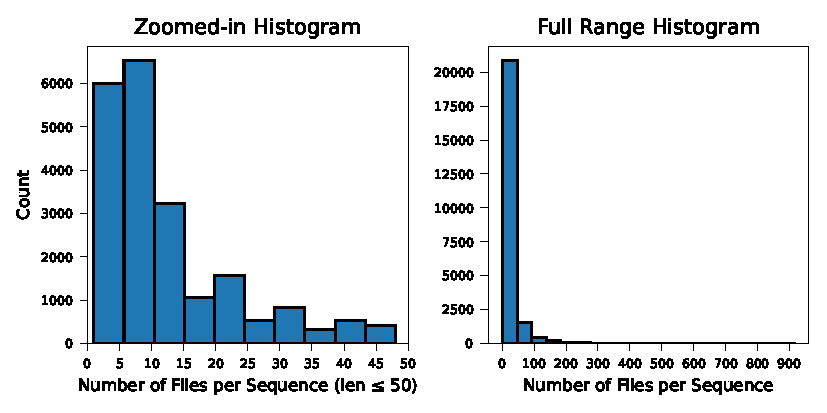
\includegraphics{figures/seq_len_histograms.pdf}
    \caption{Distribution of sequence lengths per label. More than 90\% of the sequences are between 1 and 50 images long. There are longer ones up to a length of 915 images, but these are outliers.}
    \label{fig:seq_len_histograms}
    \end{figure}

    \begin{figure}[H]
    \centering
    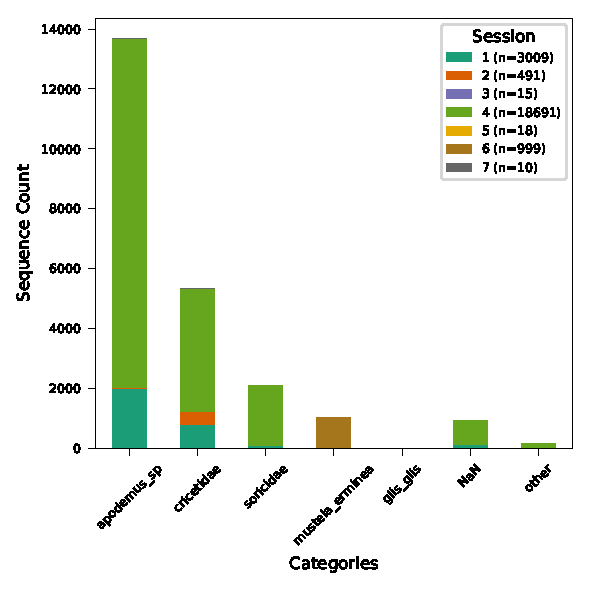
\includegraphics{figures/label2_session.pdf}
    \caption{Available sequences per label colored by session.}
    \label{fig:sequenceperlabel}
    \end{figure}

    \subsection{Data Processing}\todo{create process flow diagram}

    The data processing is divided into tree main steps: Detection, Selection, and Image Processing. 
    Further more a custom data splitting was implemented to create five stratified folds for cross-validation.
    While the detection was performed once for the whole dataset, the selection, image processing, and data splitting were implemented to be done on the fly.

        \subsubsection{Detection}
    
        In this project, the Megadetector (MD) \autocite{morrisEfficientPipelineCamera2025} is used to identify regions of interest (ROI) on all the images.
        The MD outputs a list of bounding boxe (BBox) for detected objects labeled \textit{animal}, \textit{human} or \textit{vehicle} with a corresponding confidence value.
        An example of how this detections look like is shown in \autoref{fig:detection_example}.
        This detection step was done sequence wise and the outputs were saved to json files for each sequence.

        \begin{figure}[ht]
        \centering
        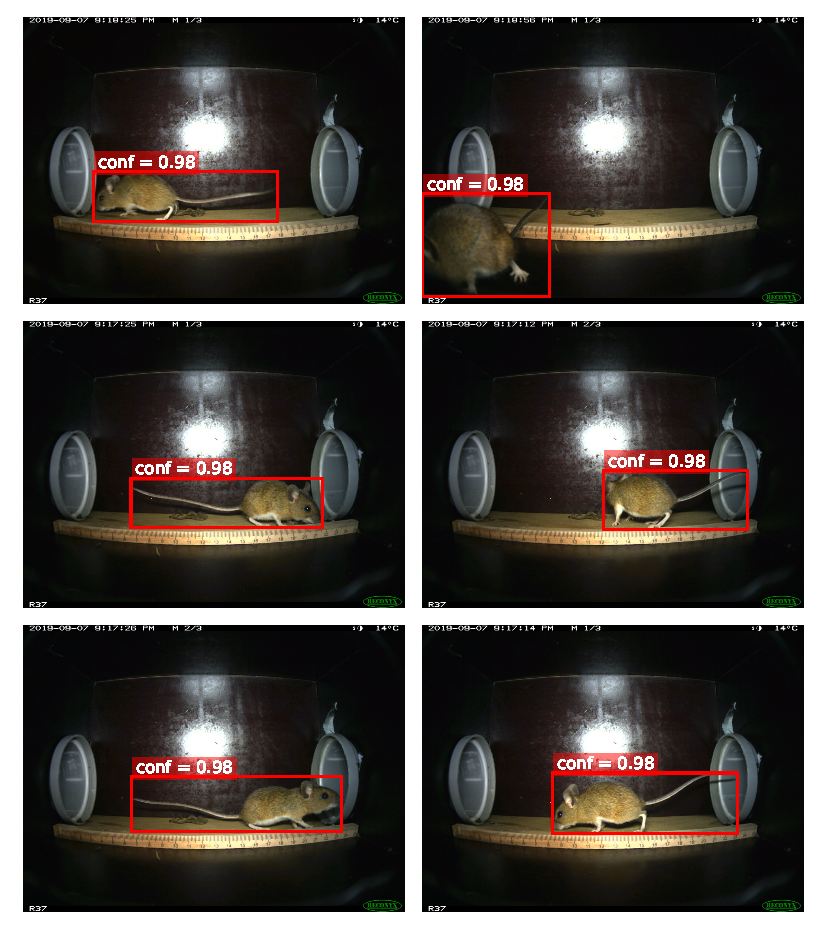
\includegraphics{figures/detections_on_a_sequence.pdf}
        \caption{Example of how the detections look like. The bounding boxes are the six highest confidence detections for the sequence 1001824 a sample from the \textit{apodemus\_sp} category.}
        \label{fig:detection_example}
        \end{figure}

        \subsubsection{Selection}
        Only images with a detection labeled \textit{animal} and a confidence score above a threshold of 0.5 where used.
        The percentage of images discarded dew to this process is shown per category in \autoref{fig:lost_images}.
        For images with multiple detections, only the BBox with the highest confidence score was considered.

        \begin{figure}[ht]
        \centering
        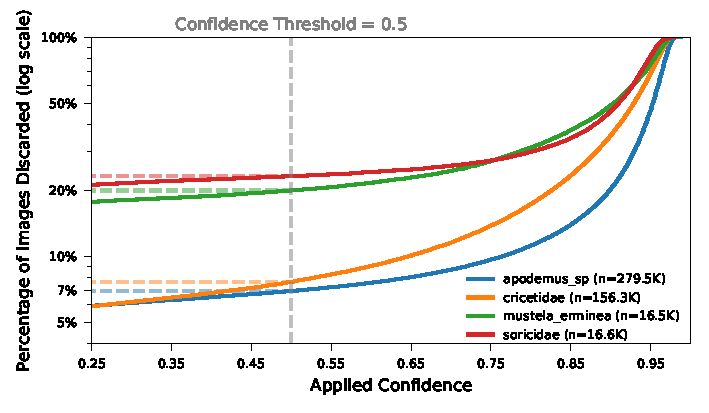
\includegraphics{figures/discarded_img_by_conf.pdf}
        \caption{Fraction of images discarded per category for a detection confidence threshold of 0.5.}
        \label{fig:lost_images}
        \end{figure}        

        \subsubsection{Image Processing}
        To process the images a custom transformation pipline was implemented using transform version 2 from the torchvision library and a custom crop function.
        This transformation was applied on the fly by the PyTorch DataLoader.
        Cropping was done using the BBoxes from the MD detection extending the BBox in order to cut the ratio expected by the model.
        In the case that the extended BBox surpasses the image border the image was padded with black pixels.
        After cropping, each image was resized to the model's expected input size, i.e.\ \(224\times224\) pixels.
        Each image was first converted into a tensor of shape \((C,H,W)\). 
        The pixel values were then normalized using the global channel wise mean and standard deviation of the dataset itself.
        This mean and standard deviation were calculated on the whole dataset, not just the training set, to ensure consistency across all folds.
        Furthermore, only the best BBox area per image was used to calculate the mean and standard deviation.

        \subsubsection{Data Splitting}
        The dataset was split into five folds using a stratified split based on the classes.
        A custom helper function was implemented to ensure the splits are done on a sequence level, meaning no sequence is ever split between folds.
        The fold size was determined by the number of images instead of the number of sequences, as the sequences vary in length.
        This approach ensures that the images are evenly distributed across the folds while maintaining the sequence integrity.
        For each class in the dataset, all the sequences were shuffled using a fixed seed for reproducibility resulting in two lists: one with the sequence ids and one with the corresponding sequence lengths.
        The list with sequence lengths was used to determine the cut-points for the folds while the list with sequence ids was used to assign the sequences to the folds.


    \subsection{Model}

    In this project, a selection of models from the torchvision library was tested to classify the images. 
    Every model was both trained from scratch and fine-tuned using the weights of a model pre-trained on ImageNet \autocite{dengImageNetLargescaleHierarchical2009}.
    A custom helper function was implemented to adapt the last layer of the model to fit the number of classes in the dataset when the model is loaded.
    The models used in this project are:

    \begin{itemize}
        \item \textbf{EfficientNet-B0} \autocite{tanEfficientNetRethinkingModel2019}:  
        A Convolutional Neural Network architecture that uses a compound scaling method to uniformly scale network width, depth, and resolution.  
        The B0 variant is the baseline model from which larger EfficientNets are derived.  

        \item \textbf{DenseNet-169} \autocite{huangDenselyConnectedConvolutional2017}:  
        A densely connected convolutional network with 169 layers in which each layer receives feature-maps from all preceding layers, fostering feature reuse and improved gradient flow.  

        \item \textbf{ResNet-50} \autocite{heDeepResidualLearning2016}:  
        A 50-layer Residual Network that introduces skip connections (residual blocks) to alleviate the vanishing-gradient problem, enabling training of very deep models.  

        \item \textbf{ViT-B\_16} \autocite{dosovitskiyImageWorth16x162021}:  
        The “Base” Vision Transformer model which splits an image into \(16\times 16\) patches, linearly embeds them, and processes the resulting sequence with a standard Transformer encoder.  
    \end{itemize}

    \subsection{Training}

    The training process was divided into four main steps repeated for each fold of the cross-validation:
    \begin{enumerate}
        \item Loading the dataset and applying the processing steps described above.
        \item Initializing the model and adapting the last layer to match the classes.
        \item Training the model for the current fold using the training set.
        \item Validating the model on the validation set and saving the best version of the model based on the lowest validation loss.
        \item The best version of the model is loaded to predict the whole dataset for later evaluation.
    \end{enumerate}

    During training, the loss was calculated using the cross-entropy loss function with the class weights calculated on the current training set.
    To adjust the model parameters, the AdamW optimizer \autocite{loshchilovDecoupledWeightDecay2019} was used with a weight decay of $10^{-5}$ and an initial learning rate of $10^{-4}$.
    The learning rate was adjusted using a cosine annealing scheduler \autocite{loshchilovSGDRStochasticGradient2017} over 50 epochs.
    A maximum of 50 epochs where trained, but an early stopping callback was implemented monitoring the validation loss with a patience of 10 epochs.
    The logging was done using the tensorboard logger, which is integrated into PyTorch Lightning and an additional custom CSV logger for easier log access for evaluation.
    A batch size of 64 was used for training -- and doubled for validation and prediction.
    Predicting the whole dataset the predicted class for each sample and the confidence scores per class were saved to a CSV file for later evaluation

    \subsection{Sequence Classification} \todo{generate a formula for this}
    Since the data is grouped into sequences and the classification was done per image, an additional step was performed to classify the sequences.
    This step was only performed after the model has been trained and the predictions for the whole dataset were available.
    To classify the sequences, the image-level predictions were aggregated by sequence ID and the confidence scores for each class were summed across all images in the sequence.
    To normalize this summed confidences, they each were divided by their sum of confidence scores.
    From this normalized confidences, the class with the highest confidence was selected as the predicted class for the sequence.
    
    % \begin{equation}
    %     S_{s,c} \;=\; \sum_{i \in s} p_{i,c}
    %     \quad,\quad
    %     \hat{S}_{s,c} \;=\; \frac{S_{s,c}}{\sum_{d=1}^{K} S_{s,d}}
    %     \quad,\quad
    %     \text{predicted\_class}(s) \;=\; \arg\max_{c}\,\hat{S}_{s,c}
    % \end{equation}

    % \noindent where:
    % \begin{description}
    % \item[$s$] is a sequence index.
    % \item[$i \in s$] iterates over all images in sequence $s$.
    % \item[$K$] is the total number of classes.
    % \item[$p_{i,c}$] is the model's confidence (probability) for class $c$ on image $i$.
    % \item[$S_{s,c}$] is the summed confidence for class $c$ over all images in sequence $s$.
    % \item[$\hat{S}_{s,c}$] is the normalized summed confidence for class $c$ in sequence $s$.
    % \item[$\text{predicted\_class}(s)$] is the class with the highest normalized summed confidence for sequence $s$.
    % \end{description}

    \subsection{Evaluation}

    The evaluation is done using the predictions created by the best version of every model for each fold.
    Both the image-level and sequence-level predictions are evaluated using the balanced accuracy (BA) score \autocite{brodersenBalancedAccuracyIts2010} as the main metric.
    The BA score is calculated using the following formula:
    \begin{equation}
    \text{BA}
    \;=\;
    \frac{1}{K} \sum_{c=1}^{K}
        \frac{TP_{c}}{\,TP_{c} + FN_{c}\,}
    \end{equation}

    \noindent where:
    \begin{description}
    \item[$K$] is the total number of classes.
    \item[$TP_{c}$] (true positives for class $c$) is the count of samples whose true label is $c$ and whose predicted label is also $c$.
    \item[$FN_{c}$] (false negatives for class $c$) is the count of samples whose true label is $c$ but whose predicted label is not $c$.
    \end{description}


    \subsection{Hardware and Software}

    This project was processed on the IUNR HPC cluster using node 301, an HPE Apollo 6500 Gen10+ node running Rocky Linux 8. 
    The node is equipped with 8 NVIDIA L40S GPUs (48 GB each), dual AMD EPYC 7742 processors, 512 cores, and 5800 GB of storage, providing the computational power needed for high-performance tasks.

    The software environment was set up using micromamba, a lightweight version of conda, to manage the dependencies and packages required for the project.
    A \textit{environment.yml} file is provided in the GitHub repository to reproduce the environment.
    The Python version and used packages are as follows:

    \begin{itemize}
        \item Python 3.10.16
        \item NumPy 2.2.4
        \item pandas 2.2.3
        \item Matplotlib 3.10.1
        \item scikit-learn 1.6.1
        \item PyTorch 2.5.1
        \item PyTorch Lightning 2.5.1
        \item Pillow 9.4.0
    \end{itemize}



% Indicate the main file. Must go at the beginning of the file.
% !TEX root = ../main.tex

%%%%%%%%%%%%%%%%%%%%%%%%%%%%%%%%%%%%%%%%%%%%%%%%%%%%%%%%%%%%%%%%%%%%%%%%%%%%%%%%
% 04_results
%%%%%%%%%%%%%%%%%%%%%%%%%%%%%%%%%%%%%%%%%%%%%%%%%%%%%%%%%%%%%%%%%%%%%%%%%%%%%%%%

\section{Results}
\label{results}

    \subsection{Detection}

    - after detection how many sequences are excluded

    - how many images are left per label

    \subsection{Classification Performance}

    All classification models did perform well on the respective test sets.
    The balanced accuracy scores for each model are shown in \autoref{tab:bal_acc_by_model}.
    The pretrained models did perform better than the models trained from scratch which is demonstrated in \autoref{fig:bal_acc_img}.
    Generally the smaller models did perform a little better than the larger models but the differences are within the standard deviation.
    The pretrained EfficientNetB0 model achieved the highest balanced accuracy of 0.992 and a standard deviation of 0.004.
    The sequence classification applied to the image classification output did improve the balanced accuracy in all cases.
    Anyhow the improvement was in the range of 0.001 to 0.005 which is again within the standard deviation.

    %==== table: overview_dataset ====%
    \begin{table}[H]
\centering
\caption{Balanced accuracy of all models -- shown as mean ± standard deviation.}
\label{tab:bal_acc_by_model}
\begin{tabular}{l c r c c}
\toprule
Model & Pretrained & Params (M) & Image BA-Score & Sequence BA-Score \\
\midrule
efficientnet\_b0 & Yes & 4 & 0.9921 ± 0.004 & 0.9947 ± 0.002 \\
densenet169 & Yes & 12 & 0.9904 ± 0.004 & 0.9939 ± 0.002 \\
resnet50 & Yes & 23 & 0.9899 ± 0.004 & 0.9934 ± 0.002 \\
vit\_b\_16 & Yes & 85 & 0.9885 ± 0.005 & 0.9933 ± 0.002 \\
\midrule
efficientnet\_b0 & No & 4 & 0.9856 ± 0.005 & 0.9898 ± 0.003 \\
densenet169 & No & 12 & 0.9863 ± 0.006 & 0.9899 ± 0.002 \\
resnet50 & No & 23 & 0.9850 ± 0.004 & 0.9888 ± 0.003 \\
vit\_b\_16 & No & 85 & 0.9767 ± 0.006 & 0.9856 ± 0.004 \\
\bottomrule
\end{tabular}
\end{table}
    %=================================%

    \begin{figure}[ht]
    \centering
    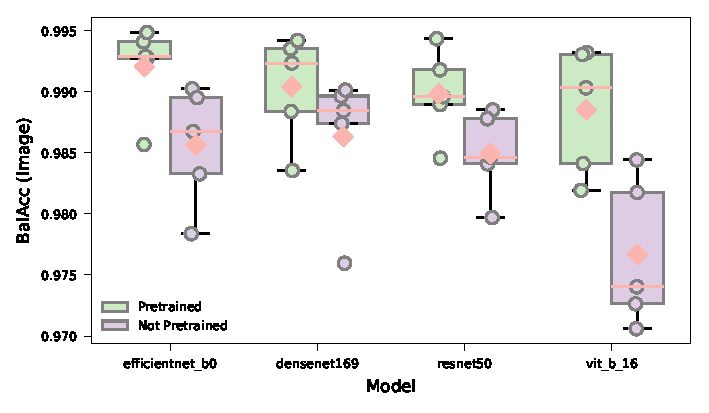
\includegraphics{figures/bal_acc_img.pdf}
    \caption{Balanced accuracy per model on the image level.}
    \label{fig:bal_acc_img}
    \end{figure}


    \subsection{Best Model}

    - More information on the best model including CM
% Indicate the main file. Must go at the beginning of the file.
% !TEX root = ../main.tex

%%%%%%%%%%%%%%%%%%%%%%%%%%%%%%%%%%%%%%%%%%%%%%%%%%%%%%%%%%%%%%%%%%%%%%%%%%%%%%%%
% 04_discussion
%%%%%%%%%%%%%%%%%%%%%%%%%%%%%%%%%%%%%%%%%%%%%%%%%%%%%%%%%%%%%%%%%%%%%%%%%%%%%%%%


\section{Discussion}
\label{discussion}

\subsection{Detection}
The detection process substantially influenced the dataset composition, particularly on the sequence level for the \texttt{mustela\_erminea} category.
This category experienced higher data loss, likely due to the relative size of the species---it is much larger than the other species captured by these MammaliaBox camera traps.
This larger size may have resulted in more frequent bad shots due to closeness to the camera or the speed at which they pass through the box---many images showed only the tip of the animal's tail disappearing out of the box.
The difficulty of properly detecting stoats using camera traps is a known issue examined, for example, by \textcite{crooseAssessingDetectabilityIrish2022}.
Another interesting observation was that the white-fur individuals were more often not detected than the brown-fur individuals.
An explanation has yet to be found for why this was only the case on the sequence level, where the \texttt{mustela\_erminea} category was disproportionately affected.
On the image level, the \texttt{soricidae} category was the most affected, with \(23\%\) of the images lost but only \(1\%\) of the sequences.

Visual inspection revealed a mixture of exemplary BBox detections alongside notable inaccuracies, such as missed detections in images with obstructions or partial visibility of animals.
Looking through misclassified images with high confidence values revealed some interesting insights.
One was that quite a few false positive detections were made, leading to surprisingly high-confidence classifications.
Some of these images were empty or contained no animal at all, as shown in \autoref{fig:false_positive_dt}, which includes examples where plant parts were misdetected, animals appeared in very dark areas, or very small, not clearly visible objects were present.
Another interesting finding was that quite a few of the images contained a snail in the highest-confidence BBox---refer to \autoref{fig:false_class_snails} for a hand-picked selection of these examples.
These misclassifications highlight the need for enhanced object discrimination capabilities or the introduction of an additional class for non-target species.

The dilemma of not missing potentially relevant detections while also not polluting the dataset with image noise remains a challenge.
Simply lowering the detection threshold to reduce missed animals is not a viable solution.
As \textcite{leornaHumanVsMachine2022} showed, reducing the \ac{MD} confidence threshold substantially increased recall, but at the cost of a profound increase in false positives, such as empty frames or vegetation.
This calls for a more sophisticated approach to reduce missed detections while maintaining a clean dataset.

\begin{figure}[ht]
\centering
\includegraphics[width=\textwidth]{figures/false_positive_dt.pdf}
\caption{Examples of false positives with high classification confidence but no animal present.}
\label{fig:false_positive_dt}
\end{figure}

\begin{figure}[ht]
\centering
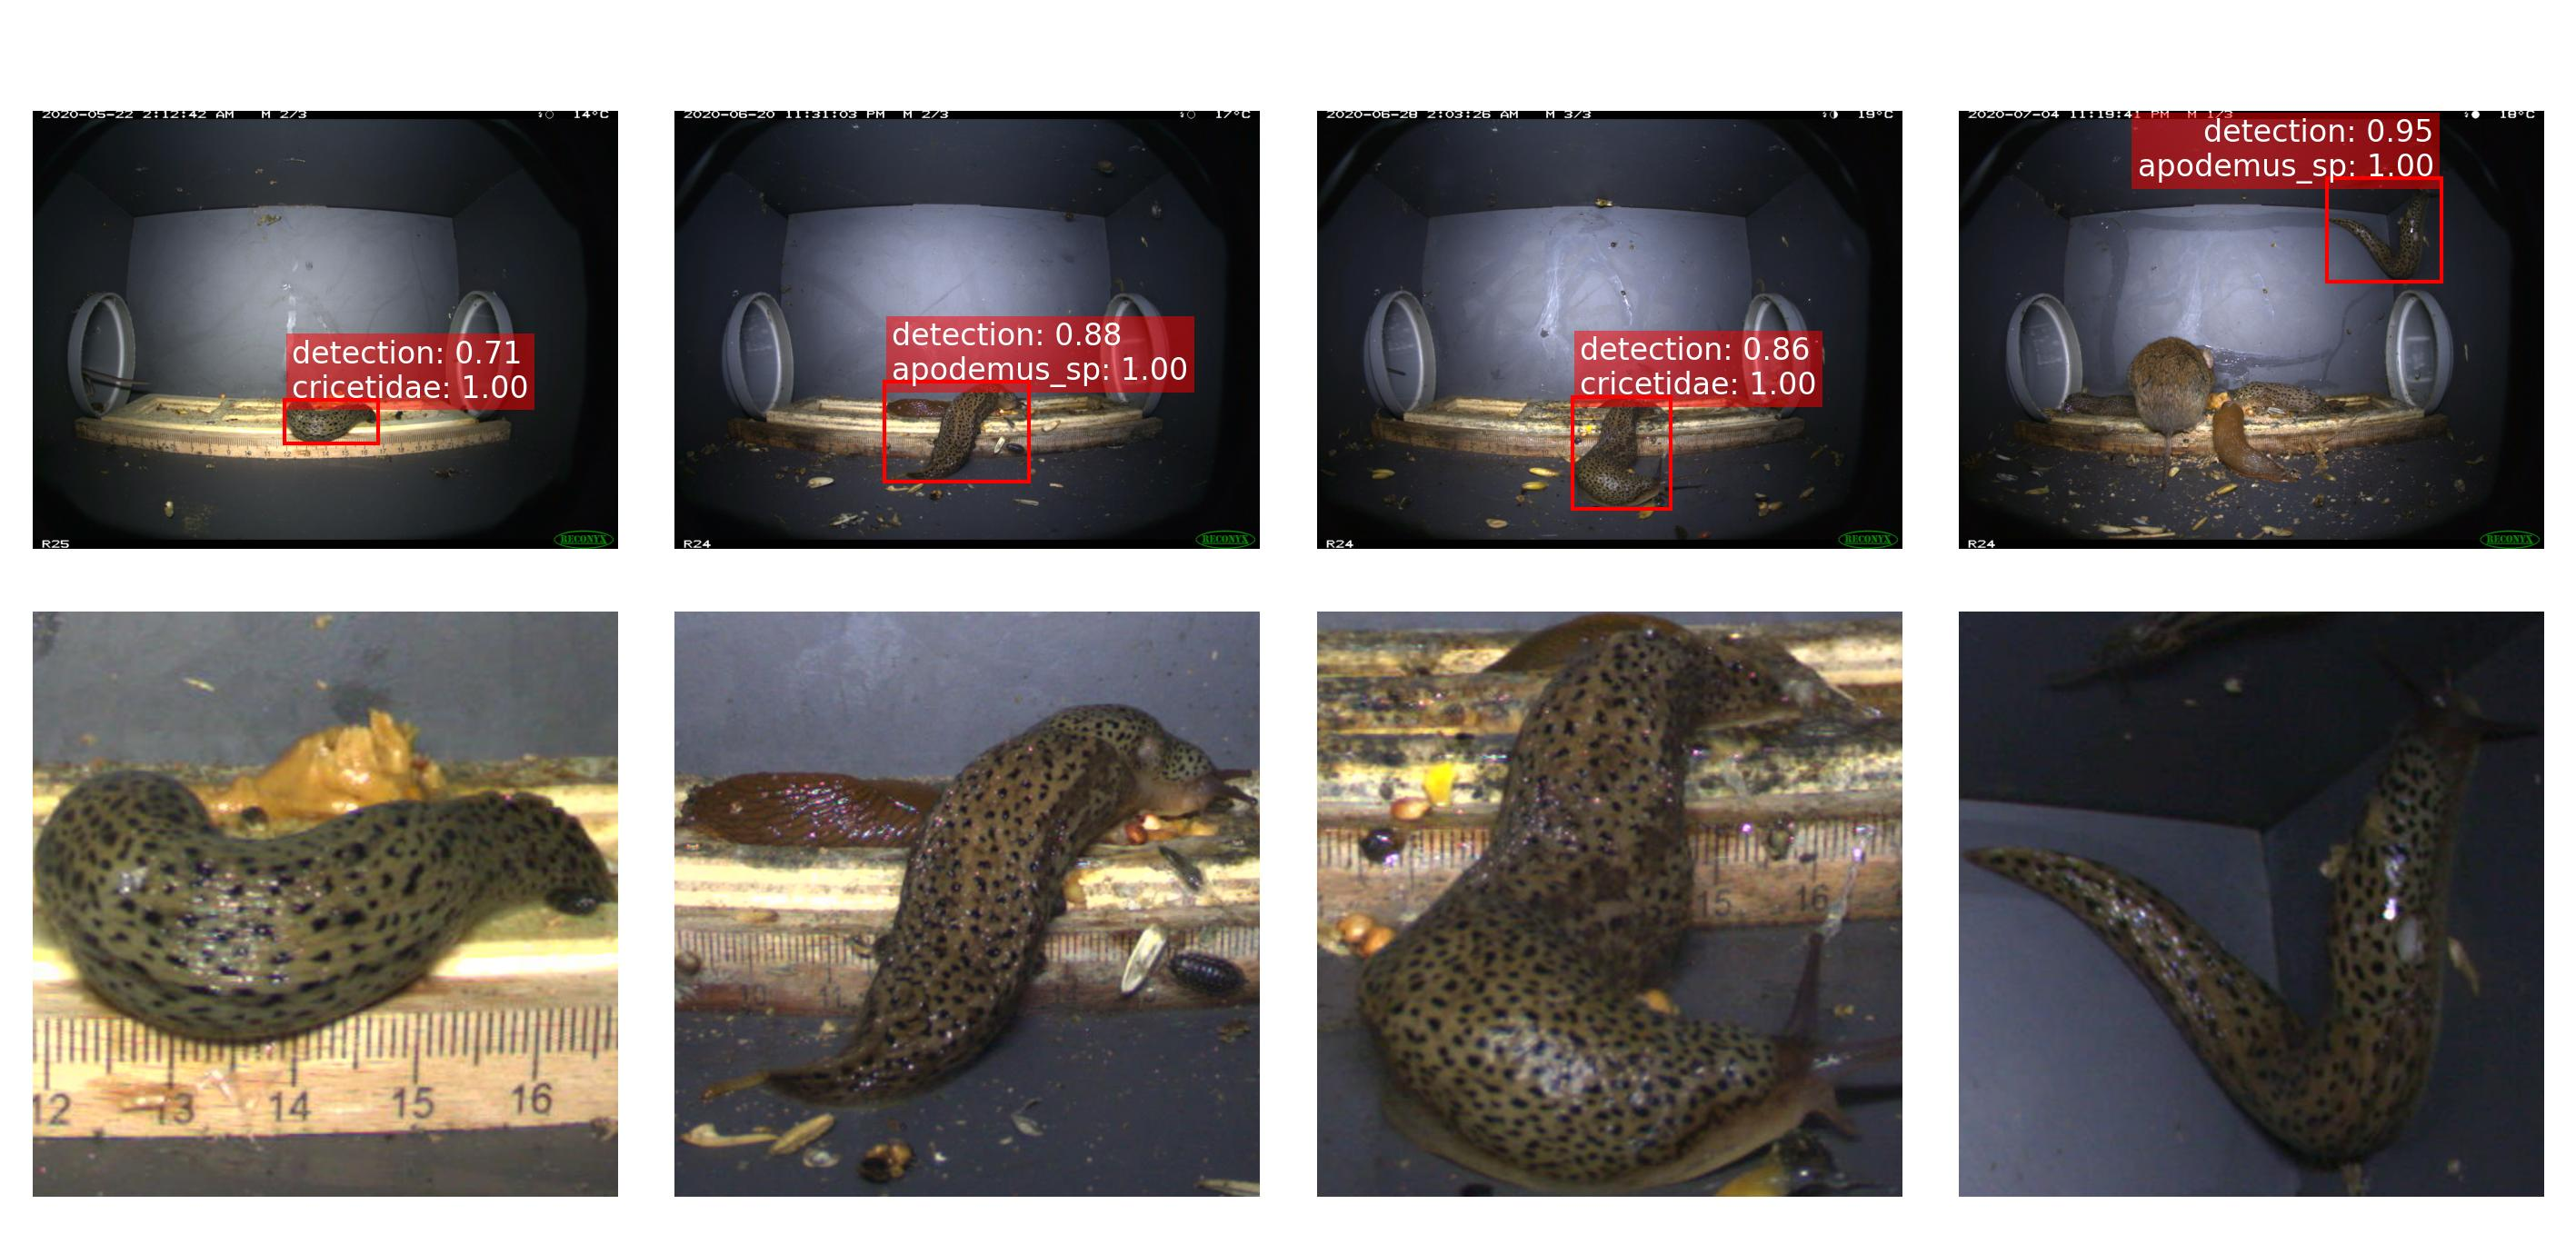
\includegraphics[width=\textwidth]{figures/false_class_snails.pdf}
\caption{Hand-picked selection of misclassified images where a snail appears in the highest-confidence BBox.}
\label{fig:false_class_snails}
\end{figure}

\subsection{Model Performance}
All tested models achieved high performance in image classification tasks, demonstrating their suitability for automating small mammal identification.
Pretrained models slightly outperformed those trained from scratch, underscoring the value of transfer learning.
The slightly better balanced accuracy of pretrained models is just one of the benefits of using pretrained models, as they also require less training time and computational resources---and hence less energy---and could potentially be trained with less data.
There are various studies exploring or applying transfer learning to camera trap images, underscoring its potential \autocite{stancicClassificationEfficiencyPreTrained2022,hopkinsDetectingMonitoringRodents2024,doanWildlifeSpeciesClassification2024,rameshExploringGeneralizabilityTransfer2025,beeryRecognitionTerraIncognita2018}.\todo{(What's the difference? Delete one?)}

Interestingly, the smaller the models, the better they performed on the image-level classification task, highlighting the fact that bigger is not always better.
Smaller models, if complex enough for the task, are always preferable since they require fewer computational resources and are faster to train.
The proper scaling of a model is an important aspect of model selection, as emphasized, for example, by \textcite{tanEfficientNetRethinkingModel2019}.
Examining \autoref{fig:bal_acc_img} again, one could speculate about a trend for smaller models to perform more consistently across folds when trained from scratch---but for some reason, this is not the case for the EfficientNet-B0 model.
The observations from this study suggest that smaller, computationally efficient models are sufficient and therefore preferable for the classification tasks at hand.


\subsection{Best Model Architecture}
The pretrained EfficientNet-B0 emerged as the best-performing architecture, achieving the highest \ac{BA}.
\autoref{fig:training_metrics_best_model} shows the validation metrics for each cross-validation fold across all epochs; note that accuracy is reported in the figure instead of \ac{BA}.
For all folds, the best version, defined by the lowest validation loss, occurred within the first few epochs, while accuracy continued to improve.
While an increase in accuracy indicates more correct predictions, the loss can still worsen because it also penalizes correct predictions made with low confidence and incorrect predictions made with high confidence.

Since the training dataset was quite large, contained only four classes and was intensively vetted using the \ac{MD}, the model was able to learn the task quite quickly.
The initial supposition that a higher detection confidence would lead to a higher classification confidence could not be confirmed by the Spearman's rank correlation coefficient.
It even suggested that the correlation is stronger for incorrect classifications.
Examining \autoref{fig:pred_conf_hexbin}, which shows the relationship between detection confidence and classification confidence, reveals that classification confidence is generally very high---across all detection confidence values and even for incorrect classifications.
There seem to be more values located in the upper right corner, which would suggest that higher detection confidence leads to higher classification confidence.
However, since there are so many samples with classification confidence close to 1 across the range of detection confidence values, Spearman's rank may not be a good measure for this relationship.

The generally high classification confidence values could be explained by the model's architecture.
In the last layers of the model, the learned features are mapped to the four classes and then normalized so the values sum to one.
If the model is entirely confident that an input does not belong to the first three classes and assigns a very small value to the fourth class (e.g., \([0\;;\;0\;;\;0\;;\;10^{-5}]\)), this distribution will be normalized to \([0\;;\;0\;;\;0\;;\;1]\), resulting in a prediction for the fourth class with maximum confidence.
As shown by \textcite{hendrycksBaselineDetectingMisclassified2018}, softmax-based confidence scores often fail to meaningfully reflect true uncertainty, especially for \ac{OOD} inputs.
Therefore, this evaluation lacks meaningfulness.
It could be repeated using logits without normalization.
Nonetheless, the assumption that a non-target class would benefit the classification task remains valid.

\begin{figure}[ht]
\centering
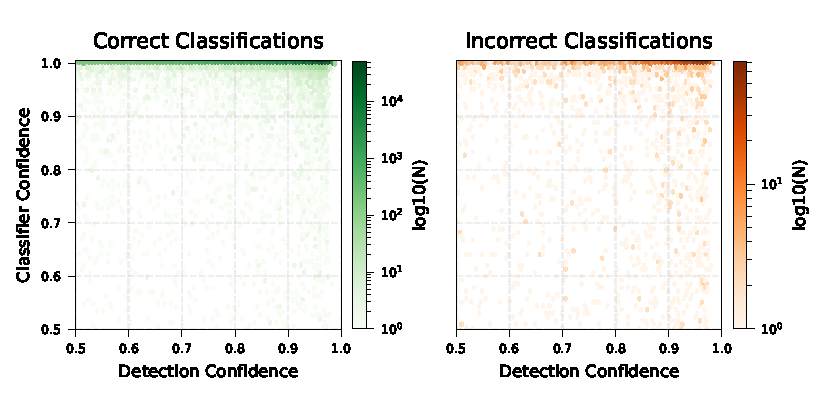
\includegraphics{figures/pred_conf_hexbin.pdf}
\caption{Hexbin plot of detection confidence vs. classification confidence for correct and incorrect predictions. Color scale indicates log$_{10}$-binned counts.}
\label{fig:pred_conf_hexbin}
\end{figure}

\subsection{Limitations}
The primary limitation of the current methodology is the absence of an explicit non-target class, forcing models into potentially incorrect predictions, particularly under \ac{OOD} conditions, exemplified by the snail misclassification issue shown in \autoref{fig:false_class_snails}.
Further, despite improvements, the \ac{MD} still misses a significant number of potentially relevant detections.
This limitation is particularly pronounced for rare species, where insufficient data reduces detection reliability.
The loss of sequences for the \texttt{mustela\_erminea} category, as shown in \autoref{tab:data_availability_after_md}, illustrates this issue.
Every sequence completely lost is a potentially missed sighting of a rare species, which could have provided valuable insights for conservation efforts.

The step of sequence classification is performed on the model's classification confidence values per class and image.
Since the information from the logits is heavily distorted by the normalization step, sequence classification does not yet reach its full potential.
This approach might need to be revisited to improve the reliability of sequence-level results.
The current approach also depends on manual preprocessing of the dataset to group the images into sequences---this process would benefit from automation.

Moreover, the current approach is heavily dependent on data availability.
Rare species inherently have fewer data points, constraining model training and potentially biasing predictions.
To include an additional class would require a sufficient number of samples to ensure reliable model performance.
Generally, data acquisition is the most resource-intensive part of most machine learning projects.


% Indicate the main file. Must go at the beginning of the file.
% !TEX root = ../main.tex

%%%%%%%%%%%%%%%%%%%%%%%%%%%%%%%%%%%%%%%%%%%%%%%%%%%%%%%%%%%%%%%%%%%%%%%%%%%%%%%%
% 05_conclusion_outlook
%%%%%%%%%%%%%%%%%%%%%%%%%%%%%%%%%%%%%%%%%%%%%%%%%%%%%%%%%%%%%%%%%%%%%%%%%%%%%%%%


\section{Conclusion and Outlook}
\label{conclusion_outlook}

\subsection{Conclusion}

This thesis demonstrated the effectiveness of deep learning models for detecting and classifying small mammals from camera trap images.
The pretrained EfficientNet-B0 model provided superior classification accuracy, quickly converging and demonstrating robustness across validation folds.
The integration of automated detections utilizing \ac{MD}, while beneficial, revealed some room for improvement, particularly concerning misdetections and missed out detections.
It was found that some finetuning of the \ac{MD} to the specific MammaliaBox camera trap setup could improve the results.
Despite these limitations, the processing pipeline and the trained models provide a promising start for developing an applicable tool and a workflow to reduce manual effort.

\subsection{Outlook}
The sequence-based classification did not improve classification performance significantly as it was done in this thesis.
It still seems a very promising approach, since camera trap images are often taken in sequences and the sequence information could be used to improve classification performance.
Further research could explore different options for sequence-based classification.
As a first step, the model's output could be evaluated on the logits level to determine how this information could be utilized to improve classification performance.
More sophisticated approaches could involve utilizing temporally aware models, as demonstrated by \textcite{muhammadTemporalSwinFPNNetNovel2024}.
Since the initial detection process using \ac{MD} could still be improved, utilizing sequence information for the detection process could be explored further.
\textcite{zotinANIMALDETECTIONUSING2019} demonstrated a promising non-\ac{DL} approach for detecting animals in camera trap images using sequence information.

Future enhancements should focus on addressing current limitations by introducing an explicit category for non-target species to improve classification accuracy and reduce false predictions with high confidence.
To allow for broader application of the model, additional categories would be needed --- such as the here explicitly ignored \textit{Glis glis}, a common small mammal in Switzerland on the \textcite{iucnIUCNRedList2025} Red List of Threatened Species.
To improve the model's robustness while adding more categories --- possibly with limited data availability --- data augmentation techniques could be implemented, as they have been shown to enhance model performance and generalization \autocite{shortenSurveyImageData2019}.

Another important step toward practical application is to develop an interface or integrated software solution.
This would allow researchers to actually use the model in their workflows for monitoring small mammal populations.
This could be done in a way that integrates manual review --- which is still necessary for reliable results --- as a means of further improving the model.
Currently, the data processing pipeline still depends on manual preprocessing of the image metadata to extract sequence information.
This step would benefit from automation to streamline the workflow --- ideally, the input for the classification task would be just the raw images as retained from the camera trap.
The only available information in the \ac{EXIF} metadata that potentially allows grouping images into sequences is the timestamp.
However, this alone is not sufficient to determine sequence length, as it does not account for the actual number of images per trigger.

Better sequence information is available visually imprinted on top of the images, which could be extracted using an \ac{OCR} model --- refer to \autoref{fig:ocr_sample}.
Since the information is imprinted on the images with high contrast and no distortion, this should be a straightforward task for an \ac{OCR} model.
The fact that the first information imprinted on the image is the timestamp — which is also available in the \ac{EXIF} metadata --- could be used to match the \ac{OCR} output with the \ac{EXIF} information to quickly determine the reliability of the \ac{OCR} output.

\begin{figure}[ht]
\centering

\includegraphics{figures/ocr_example.pdf}
\caption{Top 5\% of a camera trap image —-- it was processed with the \texttt{Tesseract} \ac{OCR} model. The output string was: \enquote{\texttt{2019-09-04 1:02:09 AM M 1/3 \#9 10\textdegree C}}.}
\label{fig:ocr_sample}
\end{figure}

% Indicate the main file. Must go at the beginning of the file.
% !TEX root = ../main.tex

%%%%%%%%%%%%%%%%%%%%%%%%%%%%%%%%%%%%%%%%%%%%%%%%%%%%%%%%%%%%%%%%%%%%%%%%%%%%%%%%
% 06_declaration
%%%%%%%%%%%%%%%%%%%%%%%%%%%%%%%%%%%%%%%%%%%%%%%%%%%%%%%%%%%%%%%%%%%%%%%%%%%%%%%%


\section{Declaration}
\label{declaration}

\subsection{Declaration of AI Usage}%%%%%%%%%%%%%%%%%%%%%%%%%%%%%%%%%%%%%%%%%%%%%%

\textbf{GitHub Copilot} was active during all coding tasks as well as text writing in this thesis.
While it was primarily intended to assist with LaTeX formatting, it also provided suggestions for the text itself.
For the actual coding tasks, it was used to help solve problems, generate code snippets and played a significant role in debugging.

\textbf{ChatGPT Model o4-mini} was used to assist with coding, problem-solving and debugging.
\textbf{ChatGPT GPT-4o} and \textbf{GPT-4.5} were used to support content research, thesis structuring, writing and refining the text.
The Abstract was initially generated and translated using \textbf{ChatGPT GPT-4o}.
Both versions where thoroughly reviewed and manually edited.
Every paragraph was finally fed into \textbf{GPT-4o} for a final spelling and grammar check --- all changes were manually reviewed using a git diff viewer to ensure that no unwanted edits were introduced.

\newpage
\refstepcounter{subsection}
\addcontentsline{toc}{subsection}{\protect\numberline{\thesubsection}Statement of Authorship}

\newgeometry{left=0in, right=0in, top=0.5in, bottom=0in}
\thispagestyle{empty}
\begin{figure}[h!]
    \centering
    
\includegraphics[width=0.9\textwidth]{appendix/declaration_independence.pdf}
\end{figure}
\restoregeometry % Restore original margins


{\sloppy
\printbibliography[heading=bibintoc]
}

% \appendix
% % Indicate the main file. Must go at the beginning of the file.
% !TEX root = ../main.tex

%%%%%%%%%%%%%%%%%%%%%%%%%%%%%%%%%%%%%%%%%%%%%%%%%%%%%%%%%%%%%%%%%%%%%%%%%%%%%%%%
% SECTION A (Appendix)
%%%%%%%%%%%%%%%%%%%%%%%%%%%%%%%%%%%%%%%%%%%%%%%%%%%%%%%%%%%%%%%%%%%%%%%%%%%%%%%%

\section{Appendix: Tables}
\label{apendix_tables}

%==== table: overview_dataset ====%
\begin{table}[H]
\centering
\caption{Balanced accuracy of all models -- shown as mean ± standard deviation.}
\label{tab:bal_acc_by_model}
\begin{tabular}{l c r c c}
\toprule
Model & Pretrained & Params (M) & Image BA-Score & Sequence BA-Score \\
\midrule
efficientnet\_b0 & Yes & 4 & 0.9921 ± 0.004 & 0.9947 ± 0.002 \\
densenet169 & Yes & 12 & 0.9904 ± 0.004 & 0.9939 ± 0.002 \\
resnet50 & Yes & 23 & 0.9899 ± 0.004 & 0.9934 ± 0.002 \\
vit\_b\_16 & Yes & 85 & 0.9885 ± 0.005 & 0.9933 ± 0.002 \\
\midrule
efficientnet\_b0 & No & 4 & 0.9856 ± 0.005 & 0.9898 ± 0.003 \\
densenet169 & No & 12 & 0.9863 ± 0.006 & 0.9899 ± 0.002 \\
resnet50 & No & 23 & 0.9850 ± 0.004 & 0.9888 ± 0.003 \\
vit\_b\_16 & No & 85 & 0.9767 ± 0.006 & 0.9856 ± 0.004 \\
\bottomrule
\end{tabular}
\end{table}
%=================================%



\end{document}  
